%% H-alpha transmission in EXHALE\_transit.py: method and implementation
%% Author: Kwang-Il Seon
\documentclass[english,a4paper]{my_memo}
\synctex=1
\usepackage{listings}
\usepackage{xcolor}
\usepackage{booktabs}

\lstset{
  basicstyle=\ttfamily\small,
  keywordstyle=\color{blue}\bfseries,
  commentstyle=\color{gray},
  stringstyle=\color{olive},
  frame=single,
  breaklines=true,
  numbers=left,
  numberstyle=\tiny\color{gray},
  language=Python
}

\usepackage{babel}

% Allow extra stretch to avoid overfull boxes from long \texttt identifiers
\setlength{\emergencystretch}{3em}

\begin{document}

\title{Transmission Spectra in EXHALE\_transit.py:\\
H$\alpha$/H$\beta$ from the Non-LTE $n=2$ Population,\\
and the Metal Resonance Doublets}
\author{Kwang-Il Seon}
\date{2026-06-12}
\maketitle

\tableofcontents
\bigskip

%=============================================================================
\section{Overview}
%=============================================================================

\texttt{EXHALE\_transit.py} (the Transmission Probability Model shipped with EXHALE)
computes transit transmission spectra by integrating the line-of-sight
(LOS) optical depth on an impact-parameter grid, using Voigt profiles
evaluated through the Faddeeva function, and then averaging over the
projected stellar disk with optional instrument and planet-rotation
convolutions. The original code handles the He\,I\,$2^3$S triplet
(10830\,\AA{}) and the H\,I / D Ly$\alpha$ doublet (1215.67\,\AA{}).

This memo documents the addition of the \textbf{H$\alpha$
(6562.8\,\AA{}, $n=2\to n=3$)} transmission spectrum. Unlike Ly$\alpha$,
which absorbs out of the ground state ($n=1$) that traces the bulk of
the atomic hydrogen, H$\alpha$ absorbs out of the $n=2$ level, whose
population must be computed from a non-LTE balance. We follow
\textbf{Christie, Arras \& Li (2013, ApJ 772, 144)}, including
collisional excitation/de-excitation, recombination cascade, two-photon
decay, $\ell$-mixing, and \textbf{Ly$\alpha$ radiative pumping}
($1s\leftrightarrow2p$). The Ly$\alpha$ mean intensity $J_{\rm Ly\alpha}(r)$
is \emph{not} produced by EXHALE; it is either read from an external text
file or, by default, estimated with the simple prescription of Huang
et~al.~(2017) --- see \S\ref{sec:jlya}.

The H$\alpha$ branch always runs; only the source of $J_{\rm Ly\alpha}$
depends on whether \texttt{Jlya\_file} is set. The existing He/Ly$\alpha$
behavior is unchanged.

This memo also documents the \textbf{metal resonance doublets}
(Mg\,II\,h\&k, Ca\,II\,H\&K, Na\,I\,D; \S\ref{sec:metals}), which are
computed by the same LOS pipeline and produce the same three-curve
spectrum figures as the H/He lines.

%=============================================================================
\section{The $n=2$ hydrogen population (Christie et~al.~2013)}
%=============================================================================

The $2s$ and $2p$ states are treated separately because they have very
different lifetimes (the $2p\to1s$ Ly$\alpha$ decay is fast,
$A_{2p\to1s}=6.3\times10^{8}\,$s$^{-1}$, whereas the $2s\to1s$ two-photon
decay is slow, $A_{2s\to1s}=8.26\,$s$^{-1}$). With $n_{1s}=n_{\rm H\,I}$,
$n_e$ and $T$ taken from the EXHALE profiles, the rate-equilibrium
equations are (Christie et~al.\ Eqs.~12--13)

\begin{align}
\bigl[A_{2p\to1s} + B_{2p\to1s}J_{\rm Ly\alpha}
   + (C_{2p\to1s}+C_{2p\to2s})n_e + \Gamma_{2p}\bigr]\,n_{2p}
   - C_{2s\to2p}\,n_e\,n_{2s}
   &= \bigl(B_{1s\to2p}J_{\rm Ly\alpha}+C_{1s\to2p}n_e\bigr)n_{1s}
      + \alpha_{2p}n_e^2, \\
\bigl[(C_{2s\to1s}+C_{2s\to2p})n_e + \Gamma_{2s} + A_{2s\to1s}\bigr]\,n_{2s}
   - C_{2p\to2s}\,n_e\,n_{2p}
   &= C_{1s\to2s}\,n_e\,n_{1s} + \alpha_{2s}n_e^2 .
\end{align}

This is a $2\times2$ linear system in $(n_{2p},n_{2s})$,
\[
\begin{pmatrix} L_{2p} & -C_{2s\to2p}n_e \\ -C_{2p\to2s}n_e & L_{2s}\end{pmatrix}
\begin{pmatrix} n_{2p}\\ n_{2s}\end{pmatrix}
=\begin{pmatrix} S_{2p}\\ S_{2s}\end{pmatrix},
\]
solved per radial cell by Cramer's rule. The total $n=2$ density driving
H$\alpha$ absorption is $n_2 = n_{2s}+n_{2p}$; in practice it is
dominated by the metastable $2s$ state.

\subsection{Rate coefficients}

The forward collisional rates are taken from Christie et~al.\ Table~2
(Janev et~al.~2003); the reverse (super-elastic) rates follow by detailed
balance using the statistical weights $g_{1s}=2$, $g_{2s}=2$, $g_{2p}=6$.
With $t_4 \equiv T/10^4\,$K:

\begin{center}
\small
\begin{tabular}{lll}
\toprule
Process & Coefficient & Expression [cm$^3$\,s$^{-1}$] \\
\midrule
Case-B recomb.\ (Draine 2011)   & $\alpha_B$        & $2.54\times10^{-13}\,t_4^{-0.8163-0.0208\ln t_4}$ \\
$\to 2s$ (incl.\ cascade)        & $\alpha_{2s}$     & $(0.282+0.047t_4-0.006t_4^2)\,\alpha_B$ \\
$\to 2p$                         & $\alpha_{2p}$     & $\alpha_B-\alpha_{2s}$ \\
$1s\to2s$ excitation             & $C_{1s\to2s}$     & $1.21\times10^{-8}\,t_4^{-0.455}\,e^{-118400/T}$ \\
$1s\to2p$ excitation             & $C_{1s\to2p}$     & $1.71\times10^{-8}\,t_4^{-0.077}\,e^{-118400/T}$ \\
$2s\leftrightarrow2p$ $\ell$-mix & $C_{2s\to2p}$     & $6.21\times10^{-5}\,(\ln(T/T_0)-\gamma)/\sqrt{T}$ \\
$2s\to1s$ (super-elastic)        & $C_{2s\to1s}$     & $1.21\times10^{-8}\,t_4^{-0.455}\,(g_{1s}/g_{2s})$ \\
$2p\to1s$ (super-elastic)        & $C_{2p\to1s}$     & $1.71\times10^{-8}\,t_4^{-0.077}\,(g_{1s}/g_{2p})$ \\
$2p\to2s$ $\ell$-mix             & $C_{2p\to2s}$     & $C_{2s\to2p}\,(g_{2s}/g_{2p})$ \\
\bottomrule
\end{tabular}
\end{center}
with $T_0=1.02\,$K and $\gamma=0.57721$ (Euler--Mascheroni). The reverse
rates are written in their analytically-cancelled form: the Boltzmann
factor $e^{+118400/T}$ implied by detailed balance cancels the
$e^{-118400/T}$ inside $C_{1s\to2s}/C_{1s\to2p}$, which avoids a
numerical $0\times\infty$ at the very low temperatures that can occur at
the base of the post-processed profile.

\subsection{Ly$\alpha$ pumping and the $J_{\rm Ly\alpha}$ input}
\label{sec:jlya}

The $1s\to2p$ pumping rate is $B_{1s\to2p}\,J_{\rm Ly\alpha}$, with the
Einstein coefficient in the mean-intensity convention
\[
  B_{1s\to2p} = \frac{g_{2p}}{g_{1s}}\,\frac{c^2}{2h\nu_{\rm Ly\alpha}^3}\,
                A_{2p\to1s} \;\simeq\; 8.55\times10^{9}\ \mathrm{cgs},
\]
and the stimulated-emission rate $B_{2p\to1s}J_{\rm Ly\alpha}$ with
$B_{2p\to1s}=(g_{1s}/g_{2p})B_{1s\to2p}$. Here $J_{\rm Ly\alpha}$ is the
\textbf{angle-averaged mean intensity $J_\nu$ at Ly$\alpha$ line center},
in cgs units $\mathrm{erg\,s^{-1}\,cm^{-2}\,Hz^{-1}\,sr^{-1}}$, so that
$B_{1s\to2p}J_{\rm Ly\alpha}$ has units of s$^{-1}$.

$J_{\rm Ly\alpha}(r)$ is obtained in one of two ways.

\paragraph{(1) From a file.} If \texttt{Jlya\_file} points to an existing
two-column text file, $J_{\rm Ly\alpha}(r)$ is read from it:
\begin{center}
\begin{tabular}{ll}
column 1 & $r/R_p$ \quad(same radial coordinate as the EXHALE output) \\
column 2 & $J_{\rm Ly\alpha}$ \quad[$\mathrm{erg\,s^{-1}\,cm^{-2}\,Hz^{-1}\,sr^{-1}}$] \\
\end{tabular}
\end{center}
\begin{sloppypar}
linearly interpolated onto the EXHALE grid and clamped to the endpoints.
A template ships as \texttt{inputdata/Jlya.txt.example}.
\end{sloppypar}

\paragraph{(2) Simple estimate (default; Huang et~al.~2017).} If no file
is given, $J_{\rm Ly\alpha}$ is estimated following Huang, Arras,
Christie \& Li (2017, ApJ 851, 150), Eq.~(6) and the surrounding text,
\[
  J_{\rm Ly\alpha}(r) \;\simeq\; 0.1\,\frac{F_{\rm LyC}}{\Delta\nu_D(r)},
  \qquad
  \Delta\nu_D = \nu_{\rm Ly\alpha}\,\frac{1}{c}\sqrt{\frac{2k_BT}{m_p}},
\]
where $\Delta\nu_D$ is the local Ly$\alpha$ Doppler width and
$F_{\rm LyC}$ is the \emph{deposited} (absorbed) Lyman-continuum energy
flux. The prefactor encodes the assumption that each LyC photoionization
is balanced by a recombination producing one Ly$\alpha$ photon; Huang
et~al.\ identify $F_{\rm LyC}$ with the total LyC flux absorbed inside
the atmosphere ($2.6\times10^{4}\,\mathrm{erg\,cm^{-2}\,s^{-1}}$ for
HD\,189733b, page~11).

\textbf{$F_{\rm LyC}$ from the actual stellar input.} Rather than a fixed
number, \texttt{EXHALE\_transit.py} computes the absorbed LyC flux from the EXHALE
inputs:
\[
  F_{\rm LyC} = \xi\,
  \underbrace{\frac{10^{\,L_{\rm EUV}}}{4\pi a^2}}_{\text{incident stellar LyC}}
  \;\times\;\underbrace{\bigl(1-e^{-\tau_{\rm LyC}}\bigr)}_{\text{fraction absorbed}},
  \qquad
  \tau_{\rm LyC} = \sigma_{\rm LyC}\,N_{\rm H\,I},
\]
where $L_{\rm EUV}$ (the EUV-band luminosity, $E>13.6$\,eV) and the
orbital distance $a$ are read from \texttt{input.inp}, $N_{\rm H\,I}$ is
the vertical neutral-hydrogen column from the EXHALE profile, and
$\sigma_{\rm LyC}\simeq6.3\times10^{-18}\,\mathrm{cm^2}$. The factor
$\xi$ is the day-night / 2D flux dilution, taken to match ATES's ``2D
approximate method'' (\texttt{Rate/2}$\to0.5$, \texttt{Rate/4}$\to0.25$,
else $1$; read from \texttt{input.inp}, cf.\ the $\xi$ factor of
Christie+2013 / Huang+2017). For the optically-thick atomic layer
$\tau_{\rm LyC}\gg1$, so the absorbed fraction $\to1$ and
$F_{\rm LyC}\to\xi\times$ the incident stellar LyC flux (e.g.\
$\xi=0.5$, $\simeq5.2\times10^{2}\,\mathrm{erg\,cm^{-2}\,s^{-1}}$ for the
HD\,209458b input). A fixed value can be forced via
\texttt{F\_LyC\_override} and the dilution via \texttt{xi\_override}.

This estimate is a uniform-illumination approximation: it omits the
decline of $J_{\rm Ly\alpha}$ deep in the atmosphere captured by the full
radiative-transfer treatment (Huang et~al.\ Eq.~7) and the direct stellar
Ly$\alpha$ component; for a self-consistent profile, supply
\texttt{Jlya\_file}.

\subsection{$n=2$ photoionization $\Gamma_{2s},\Gamma_{2p}$ (Balmer continuum)}
\label{sec:gamma2}

The $n=2$ levels are photoionized by the stellar Balmer continuum
($E>3.4$\,eV, $\lambda<3647$\,\AA{}); this depletes $n_2$ and is included
in Eqs.~(12)--(13) through $\Gamma_{2s},\Gamma_{2p}$. The Balmer-continuum
field is outside EXHALE's XUV scope, so it is estimated from a diluted
stellar blackbody: for a stellar effective temperature \texttt{T\_star}
and radius \texttt{R\_star},
\[
  \Gamma_2 = \int_{\nu_2}^{\infty}\frac{F_\nu}{h\nu}\,\sigma_2(\nu)\,d\nu,
  \quad F_\nu = \pi B_\nu(T_\star)\Bigl(\frac{R_\star}{a}\Bigr)^2,
  \quad \sigma_2(\nu)=\sigma_{2,\rm th}\Bigl(\frac{\nu_2}{\nu}\Bigr)^{3},
\]
with $\nu_2$ the $n=2$ threshold and $\sigma_{2,\rm th}\simeq1.4\times
10^{-17}\,\mathrm{cm^2}$, and $\Gamma_{2s}\simeq\Gamma_{2p}\simeq\Gamma_2$.
This reproduces Huang et~al.'s Table~2 values ($\sim20$--$26\,$s$^{-1}$)
for a K dwarf, and is substantially larger for a hotter G dwarf
(e.g.\ $\sim140\,$s$^{-1}$ for HD\,209458's $T_\star\simeq6065\,$K), which
suppresses $n_2$ and hence the Balmer-line depth. Setting
\texttt{T\_star}$\le0$ falls back to the manual constants
\texttt{Gamma\_2s}/\texttt{Gamma\_2p} (default $0$).

%=============================================================================
\section{H$\alpha$ and H$\beta$ optical depth and transmission}
%=============================================================================

Once $n_2(r)$ is known, the H$\alpha$ transmission is computed with the
same LOS integration as Ly$\alpha$. Along a chord at impact parameter $b$,
\[
  \tau_\nu(b) = \int n_2(r)\,\sigma_{\rm H\alpha}(\nu,r)\,d\ell,
  \qquad
  \sigma_{\rm H\alpha} = \frac{\sqrt{\pi}\,e^2}{4\pi\epsilon_0 m_e c}\,
  \frac{f_{23}}{\Delta\nu_D}\,H(a,x),
\]
where $H(a,x)=\mathrm{Re}\,[w(x+ia)]$ is the Voigt function (Faddeeva
$w$), $\Delta\nu_D=\nu_{\rm H\alpha}v_{\rm th}/c$ uses the proton thermal
speed, and the line-of-sight bulk velocity is folded into $x$ exactly as
for the existing lines. Atomic data: $\lambda_{\rm H\alpha}=6562.8\,$\AA{}
(air), $f_{23}=0.6407$, $A_{3\to2}=4.41\times10^{7}\,$s$^{-1}$ (the line
is strongly Doppler-dominated, so the damping wing is negligible). The
disk-averaged transmission, instrument convolution and planet-rotation
convolution reuse the existing code paths.

\paragraph{H$\beta$ ($n=2\to n=4$).} The same $n=2$ population also
produces H$\beta$ at $\lambda_{\rm H\beta}=4861.35\,$\AA{} ($f_{24}=0.119$,
$A_{4\to2}=8.42\times10^{6}\,$s$^{-1}$). It is computed with an identical
LOS loop and plotted/printed alongside H$\alpha$. Because both lines are
%% STALE (P48; Update_EXHALE section 137): computed with the profile files' GHOST
%% rows included -- the two boundary rows at each end of every Hydro_ioniz /
%% Ion_species file, which the Python readers now drop. Measured shift on three
%% states: 0.2--3.8 per cent on the line-center and 4 A band depths. Values left
%% exactly as measured; regeneration awaits instruction.
optically thick (saturated), the H$\alpha$/H$\beta$ depth ratio is much
smaller than the optical-depth ratio ($\sim7.3$): e.g.\ on the converged
HD\,209458b run, H$\alpha\simeq3.2\%$ and H$\beta\simeq2.0\%$ with TPM's
default star, and $\simeq0.41\%$ / $0.26\%$ with HD\,209458's actual
$R_\star,T_\star$ (see the comparison notebook).

%=============================================================================
\section{Implementation in \texttt{EXHALE\_transit.py}}
%=============================================================================

\paragraph{System parameters.} The planet and the star are taken from the run
directory, matched by label exactly as \texttt{input\_read.f90} does. Besides
$R_p$, $M_p$, $T_{\rm eq}$, $a$,
$M_\star$, $L_{\rm EUV}$ and the 2-D approximate method, this includes the
stellar radius (\texttt{Stellar radius [R\_sun]}) and effective temperature
(\texttt{Stellar Teff [K]}), which set the transit normalization $A_\star$,
the $R_\star/R_p$ cap on the absorbing annulus, and the diluted-blackbody
Balmer continuum of \S\ref{sec:gamma2}. The planet spin period has no
\texttt{input.inp} key: a close-in giant is tidally locked, so it defaults to
the Keplerian orbital period $P_{\rm orb}=2\pi\sqrt{a^3/[G(M_\star+M_p)]}$.
Each of the three is resolved as \texttt{EXHALE\_TRANSIT\_RSTAR\_RSUN} /
\texttt{\_TSTAR} / \texttt{\_ROTP} environment override $>$
\texttt{./input.inp} $>$ built-in default, and the resolved values and their
sources are printed at startup.

\paragraph{\texttt{EXHALE\_resolved.out} comes first (2026-08-22).} $R_p$,
$M_p$, $T_{\rm eq}$, $a$, $M_\star$ and He/H are read from
\texttt{EXHALE\_resolved.out} beside \texttt{input.inp} whenever that file
exists, and only from \texttt{input.inp} when it does not. The wind solver
writes it (\texttt{write\_resolved\_config} in
\texttt{write\_setup\_report.f90}) \emph{after} a \texttt{base.inp} handoff or a
lower-atmosphere profile has moved the base, so it is the geometry the wind
actually used, while \texttt{input.inp} alone is stale in exactly that case.
\texttt{read\_input\_params} says at startup which of the two it took, and a
file that is present but unreadable raises rather than falling back silently.
The stellar radius and $T_{\rm eff}$ are not in that file and keep the
precedence above.

\begin{itemize}
  \item \texttt{n2\_populations(T,n1s,nHII,ne,Jlya,G2s,G2p)} solves the
    $2\times2$ system above and returns $(n_{2s},n_{2p},n_2)$ in
    cm$^{-3}$. The Ly$\alpha$-pump constants $B_{1s\to2p}$, $B_{2p\to1s}$
    are precomputed.
  \item $J_{\rm Ly\alpha}$ is read from \texttt{Jlya\_file} if present,
    otherwise built from the Huang et~al.~(2017) estimate
    (\S\ref{sec:jlya}); $n_2$ is then built into the symmetric
    (inverted$+$normal) radial profile \texttt{data\_n2} (in m$^{-3}$),
    exactly like \texttt{data\_nHI}.
  \item A new wavelength grid \texttt{l\_onde\_Ha} and an H$\alpha$ LOS
    loop fill \texttt{exp\_tau\_Ha}; the disk average, instrument
    convolution (\texttt{Instr\_res\_Ha}) and rotation convolution
    produce the plotted curves.
  \item The H$\alpha$ branch always runs (\texttt{do\_Ha=True}); with the
    default \texttt{Jlya\_file=''} it uses the Huang et~al.~(2017)
    estimate for $J_{\rm Ly\alpha}$, with $F_{\rm LyC}$ taken as the
    absorbed stellar LyC flux (\S\ref{sec:jlya}).
  \item \textbf{Compatibility fix.} \texttt{Ion\_species.txt} in
    EXHALE carries trace-metal columns, so the
    reader was changed to \texttt{usecols=range(7)} to take only
    $r$ and the six H/He species. This also remains correct for the old
    13-column (C/O-only) and 7-column (H/He-only) outputs.
    The column count has since grown: \texttt{write\_output.f90} writes $r$,
    the six H/He species (\texttt{HI HII HeI HeII HeIII HeITR}) and all
    \texttt{n\_mion} $=27$ metal-ion stages, i.e.\ \textbf{34} columns, and
    \textbf{38} on a molecular run, which appends \texttt{H2 H2p H3p HeHp}; the
    metal columns are written whether or not metals are on. The
    \texttt{usecols=range(7)} slice is unaffected --- the first seven columns
    are still $r$ plus the six H/He species --- and anything past them is found
    through the file's own \texttt{\# columns} schema header.
\end{itemize}

\subsection{Outputs}\label{sec:outputs}

Every line carries one key --- \texttt{He10830}, \texttt{Lya},
\texttt{Halpha}, \texttt{Hbeta}, \texttt{MgII}, \texttt{CaII},
\texttt{NaI} --- and both products of a line are named from that key and
land in the run directory:

\begin{center}
\begin{tabular}{@{}lll@{}}
\hline
Product & Name & Default \\
\hline
model curve & \texttt{<path>/tpm\_<line>.txt} & always written \\
figure & \texttt{<path>/<prefix><line>.png} ($+$ \texttt{.pdf})
        & off; set \texttt{EXHALE\_TRANSIT\_FIG\_PREFIX} \\
\hline
\end{tabular}
\end{center}

\noindent A curve file has the columns \texttt{lambda[A]}, $T_\lambda$
(theoretical), $T_\lambda$ (instrument-convolved), $T_\lambda$
($+$rotation), so the excess absorption in percent is
$(1-T_\lambda)\times100$. The set follows the run: a metals-off run
writes no metal curves. \texttt{EXHALE\_TRANSIT\_SAVE\_PREFIX} decorates
the curve name exactly as the figure prefix decorates the figure name,
and both are resolved against the run directory, so an absolute prefix
writes elsewhere and nothing depends on the working directory.

%=============================================================================
\section{Validation}
%=============================================================================

%% STALE (P48; Update_EXHALE section 137): computed with the profile files' GHOST
%% rows included -- the two boundary rows at each end of every Hydro_ioniz /
%% Ion_species file, which the Python readers now drop. Measured shift on three
%% states: 0.2--3.8 per cent on the line-center and 4 A band depths. Values left
%% exactly as measured; regeneration awaits instruction.
Run end-to-end on the converged HD\,209458b EXHALE output
(\texttt{output/*\_adv.txt}), the module is stable and \texttt{NaN}-free
and yields clean H$\alpha$ and H$\beta$ absorption lines at $6562.8$ and
$4861.4$\,\AA{}. With the Huang $J_{\rm Ly\alpha}$ estimate
($\xi=0.5$, $F_{\rm LyC}\simeq5.2\times10^{2}$, $\Gamma_2$ from
$T_\star=6065\,$K), the depths are physically reasonable and the
H$\alpha$/H$\beta$ ratio reflects saturation (both optically thick). The
Ly$\alpha$ branch in the same run saturates ($\sim100\%$ core absorption)
and He\,I behaves as before. A worked comparison against the
Jensen et~al.~(2012) HD\,209458b observation is provided in the notebook
\texttt{Halpha\_compare\_HD209458b.ipynb}.

%=============================================================================
\section{Metal resonance doublets (Mg II h\&k, Ca II H\&K, Na I D)}
\label{sec:metals}
%=============================================================================

The metal resonance lines are the key NUV/optical diagnostics of
metal-enriched escaping atmospheres (Huang et~al.~2023). They absorb out
of the \emph{ion ground state}, whose excited fine-structure levels are
Boltzmann-negligible at $\sim10^4$\,K, so the lower-level density is the
ion density itself ($n_{\rm lower}\simeq n_{\rm ion}$) --- no non-LTE
population calculation is needed. The ion-density profiles are read from
the metal block of \texttt{Ion\_species\_adv.txt}; a metals-off run
(all-zero columns) skips this section automatically.

\subsection{Atomic data and implementation}

Each species is treated as a \textbf{doublet}, with both components
summed in a single wavelength window
(Table~\ref{tab:metal-lines}; NIST $f$-values and $A$-coefficients).
The optical depth uses exactly the H/He pipeline: spherical chords
$\sqrt{r^2-b^2}$ on the impact-parameter grid, LOS velocity
$v_{\rm los}=v\,x/r$, Voigt profiles via the Faddeeva function
(vectorized over wavelength), trapezoidal $\tau$, projected-area disk
average, then the instrument convolution and the planet-rotation
convolution with the depth-dependent effective radius
$R_{\rm eff}=R_p\sqrt{(h+\delta)/\delta}$ (capped at the
impact-parameter boundary), $\delta=(R_p/R_\star)^2$. The three doublets
are written under the same \texttt{tpm\_<line>} naming as the H/He lines
(\S\ref{sec:outputs}), with the keys \texttt{MgII}, \texttt{CaII},
\texttt{NaI}.

\begin{table}[htbp]
\centering\small
\caption{Metal resonance doublets in \texttt{EXHALE\_transit.py} (NIST).}
\label{tab:metal-lines}
\begin{tabular}{llcccl}
\toprule
species & component & $\lambda_0$ [\AA{}] & $f$ & $A_{21}$ [s$^{-1}$] & window / $R_{\rm instr}$ \\
\midrule
Mg\,II & k & 2796.352 & 0.608 & $2.60\times10^8$ &
  2790--2810\,\AA{} / $3\times10^4$ \\
       & h & 2803.531 & 0.303 & $2.57\times10^8$ & \\
Ca\,II & K & 3933.663 & 0.6267 & $1.47\times10^8$ &
  3927--3975\,\AA{} / \texttt{Instr\_res\_Ha} \\
       & H & 3968.469 & 0.3116 & $1.40\times10^8$ & \\
Na\,I  & D2 & 5889.951 & 0.641 & $6.16\times10^7$ &
  5884--5902\,\AA{} / \texttt{Instr\_res\_Ha} \\
       & D1 & 5895.924 & 0.320 & $6.14\times10^7$ & \\
\bottomrule
\end{tabular}
\end{table}

Alongside the spectra, the script prints the validated
\emph{single-component} depth table (line-center and 4\,\AA{}-band
percentages for Mg\,II\,2796, Ca\,II\,K, Na\,I\,D2), which is the
quantity used for the Huang et~al.~(2023) comparisons; the doublet peak
differs from the single-component value only by the partner-line wing
(e.g.\ 3.75 vs.\ 3.72\% for Mg\,II on WASP-121b). Two conventions
matter when comparing with Huang: their table lists the effective
transit radius $R_{\rm eff}/R_\star=\sqrt{(R_p/R_\star)^2+h}$, not a
percent absorption, and Mg\,II is quoted in a 4\,\AA{} NUV bin while the
optical lines are line-center (line-center vs.\ 4\,\AA{} differ by
$\sim3\times$ for the optically thick Mg\,II core).

For a Roche-lobe run the 3-D equipotential reconstruction
(\texttt{geometry = 'triaxial'}, \texttt{roche\_recon.py}) replaces the
spherical chords by the full Roche geometry with an LOS velocity for each sector
$v_{\rm sub}(r_{\rm eff})\,x/r-\Omega y$ (wind $+$ tidally locked
rotation) and reports the same depth table.

\subsection{Example spectra}

%% STALE (P48; Update_EXHALE section 137): computed with the profile files' GHOST
%% rows included -- the two boundary rows at each end of every Hydro_ioniz /
%% Ion_species file, which the Python readers now drop. Measured shift on three
%% states: 0.2--3.8 per cent on the line-center and 4 A band depths. Values left
%% exactly as measured; regeneration awaits instruction.
Figure~\ref{fig:metalspec} shows the three doublet spectra for the
WASP-121b worked example (\texttt{backup/regression/tpm\_wasp/}, Roche Newton
solution, metals on). The optically thick cores saturate, so the two
doublet members reach similar depths despite the 2:1 oscillator-strength
ratio; the rotation convolution mainly shallows and broadens the narrow
Na\,I\,D cores.

\begin{figure}[htbp]
\centering
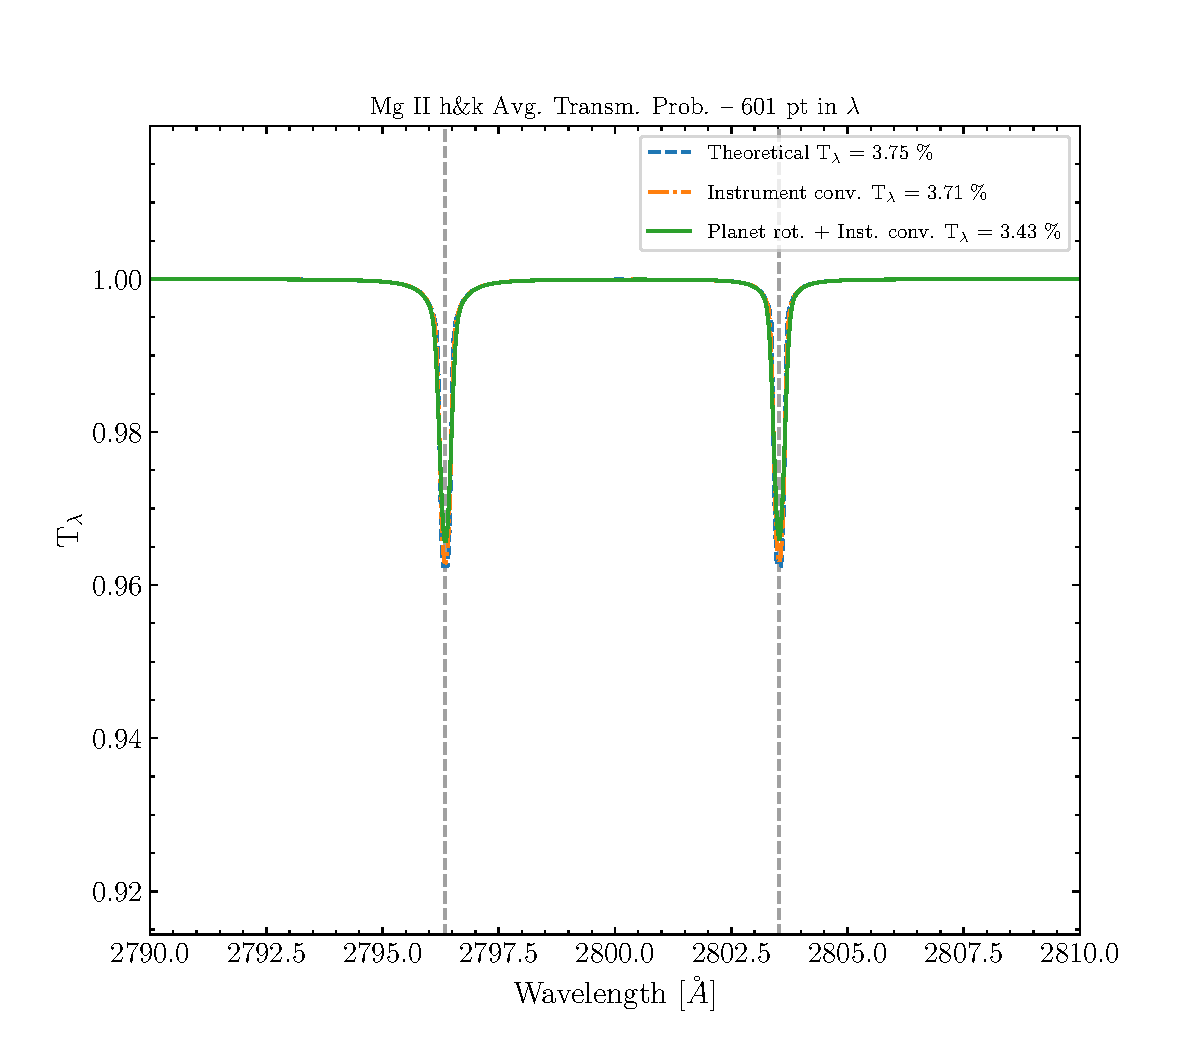
\includegraphics[width=0.49\textwidth]{figures/tpm_MgII.pdf}\hfill
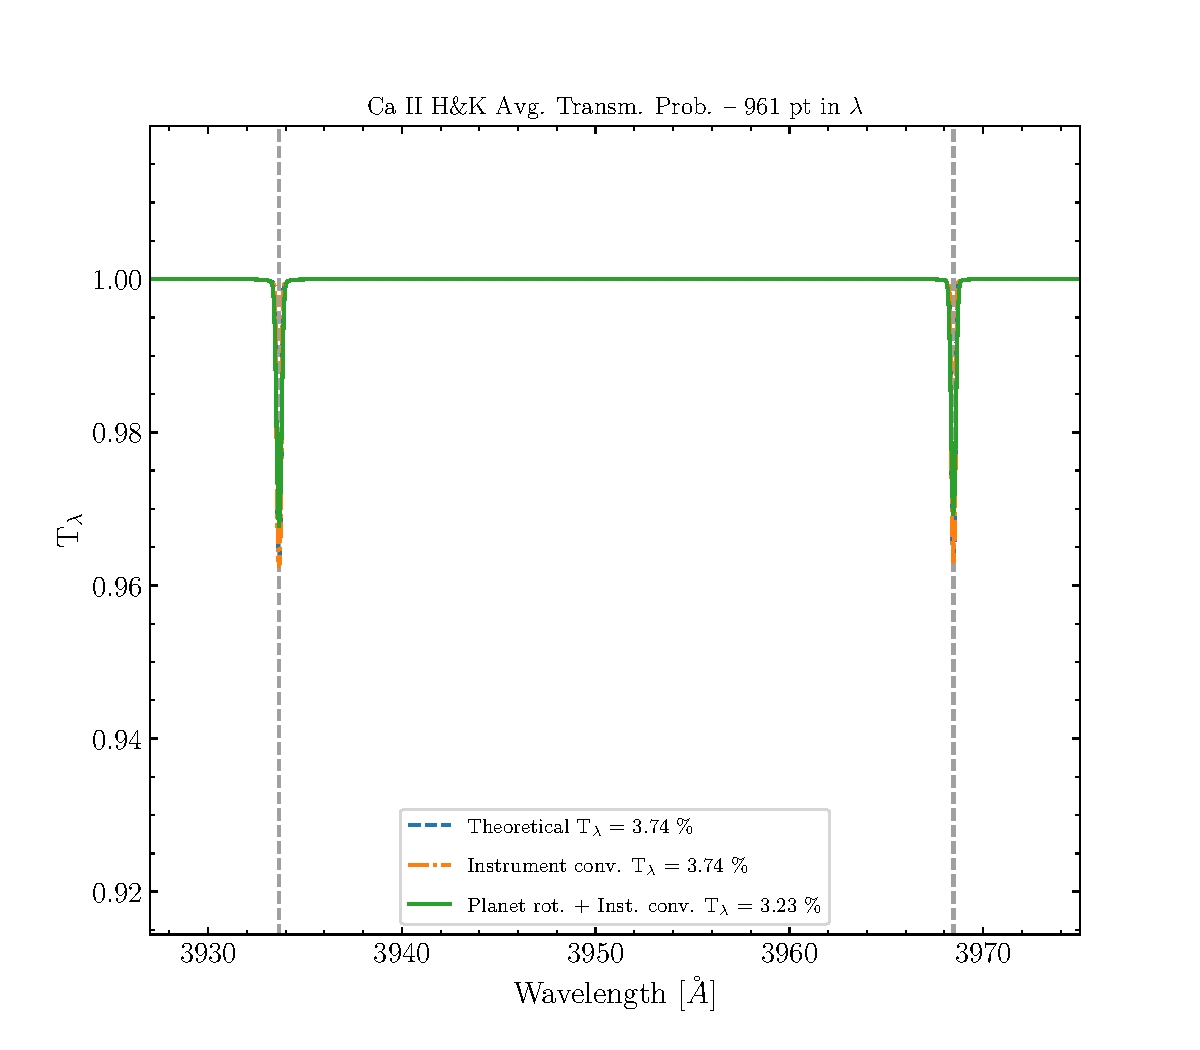
\includegraphics[width=0.49\textwidth]{figures/tpm_CaII.pdf}\\[2pt]
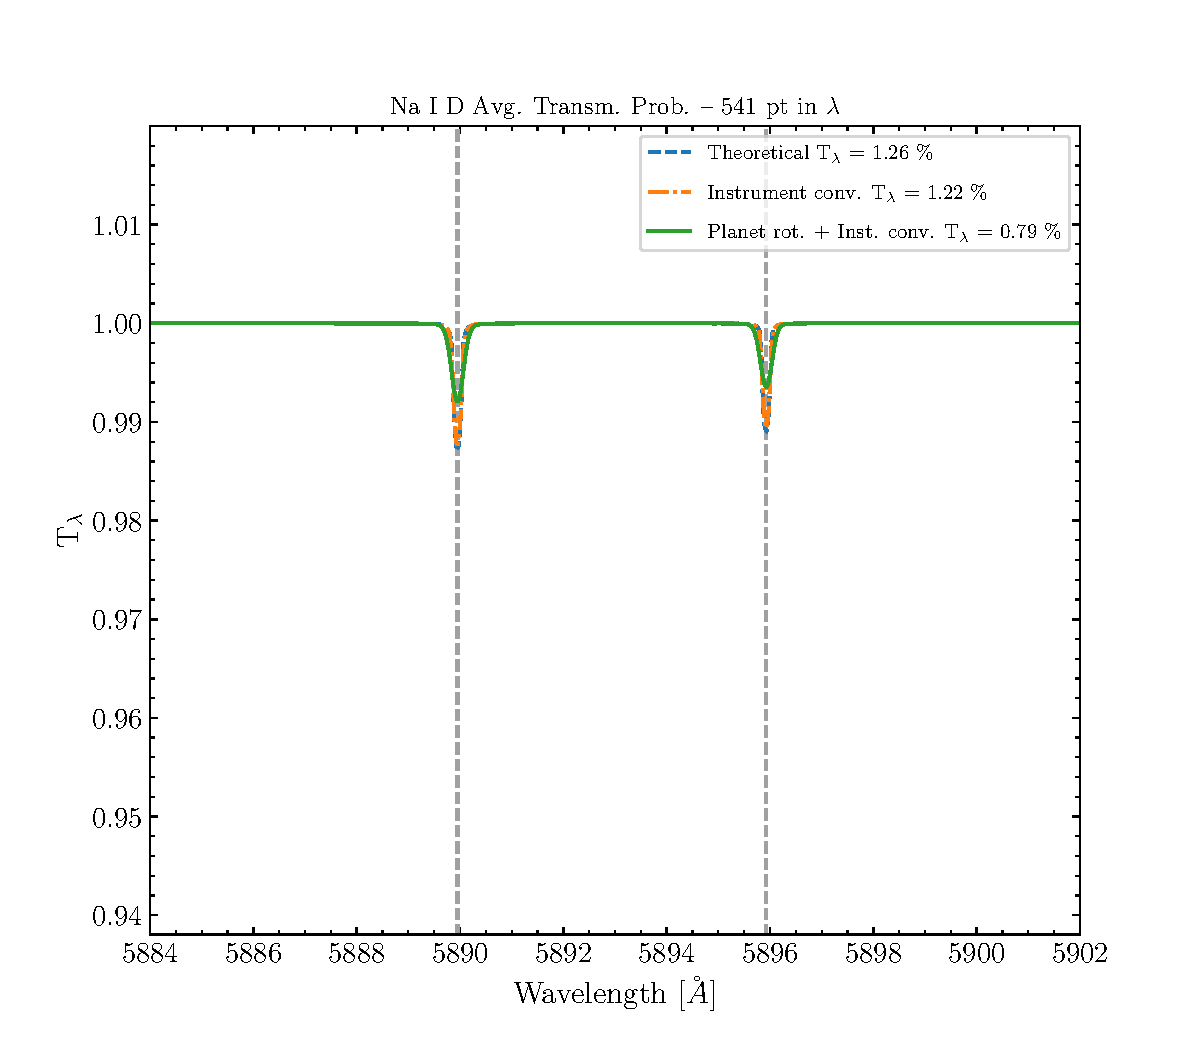
\includegraphics[width=0.49\textwidth]{figures/tpm_NaI.pdf}
\caption{Metal resonance doublet transmission spectra for WASP-121b
(\texttt{backup/regression/tpm\_wasp/}): Mg\,II\,h\&k (top left),
Ca\,II\,H\&K (top right), and Na\,I\,D (bottom). Each panel shows the
theoretical, instrument-convolved, and instrument$+$rotation-convolved
transmission, as for the H/He lines.}
\label{fig:metalspec}
\end{figure}

%=============================================================================
\section{Caveats}
%=============================================================================

\begin{enumerate}
  \item \textbf{$n=2$ photoionization.} $\Gamma_{2s},\Gamma_{2p}$ are now
    estimated from a diluted stellar-blackbody Balmer continuum
    (\S\ref{sec:gamma2}, parameter \texttt{T\_star}); this is a single
    blackbody approximation to the true stellar near-UV spectrum. Setting
    \texttt{T\_star}$\le0$ reverts to the manual constants (default $0$).
  \item \textbf{Electron density.} $n_e=n_{\rm H\,II}+n_{\rm He\,II}
    +2n_{\rm He\,III}$ from EXHALE is used (Christie assume $n_e=n_p$); the
    difference is small.
  \item \textbf{$J_{\rm Ly\alpha}$ convention.} The input must be the
    mean intensity $J_\nu$ at line center in cgs (\S\ref{sec:jlya}). A
    different convention (energy density, frequency-integrated, etc.)
    requires rescaling the pump constant.
  \item \textbf{Wavelength/damping.} $\lambda_{\rm H\alpha}$ is the air
    value 6562.8\,\AA{}; the natural width is negligible relative to the
    thermal Doppler width, so the line is essentially Gaussian.
\end{enumerate}

%=============================================================================
\section*{Reference}
%=============================================================================
\noindent Christie, D., Arras, P., \& Li, Z.-Y.\ 2013, ApJ, 772, 144 ---
``H$\alpha$ Absorption in Transiting Exoplanet Atmospheres''
(\texttt{references/Christie\_2013ApJ\_772\_144.pdf}).

\medskip
\noindent Huang, C., Arras, P., Christie, D., \& Li, Z.-Y.\ 2017, ApJ,
851, 150 --- ``A Model of the H$\alpha$ and Na Transmission Spectrum of
HD\,189733b'' (\texttt{references/Huang\_2017\_ApJ\_851\_150.pdf});
the $J_{\rm Ly\alpha}$ estimate is their Eq.~(6) and related text.

\medskip
\noindent Jensen, A.~G., et~al.\ 2012, ApJ, 751, 86 --- transit H$\alpha$
spectroscopy of HD\,209458b and HD\,189733b (comparison target for the
HD\,209458b notebook).

\end{document}
